\section{Performance Benchmarking}\label{sec:results}

Our research has conducted extensive benchmarking of GASing implementations across multiple programming languages and against standard arithmetic libraries. The benchmarking framework tests:

\begin{itemize}
    \item Different input sizes (from small to very large integers)
    \item Various input patterns (random, repeated digits, etc.)
    \item Implementation variations (pure Python, C bindings, Rust bindings)
    \item Comparison with specialized libraries (mpmath, sympy, gmpy2)
\end{itemize}

\subsection{Addition Performance}

Our addition performance benchmarks reveal several key insights:

\begin{enumerate}
    \item For small numbers ($<$100 digits), specialized libraries like gmpy2 consistently outperform GASing implementations
    \item For medium-range numbers (100-1000 digits), optimized GASing implementations in C and Rust show competitive performance
    \item For specific patterns (e.g., repeated digits), pattern-optimized GASing implementations occasionally outperform general-purpose libraries
\end{enumerate}

\begin{table}[h]
\centering
\caption{Relative Performance for 100-digit Addition Operations}
\label{tab:addition_performance}
\begin{tabular}{lcc}
\toprule
\textbf{Implementation} & \textbf{Time (ns)} & \textbf{Relative Performance} \\
\midrule
gmpy2\_addition & 543 & 1.00x (baseline) \\
gasing\_add\_rust\_optimized & 892 & 1.64x slower \\
mpmath\_addition & 1,254 & 2.31x slower \\
sympy\_addition & 1,893 & 3.49x slower \\
gasing\_simulasi & 2,341 & 4.31x slower \\
penjumlahan\_tradisional & 3,572 & 6.58x slower \\
\bottomrule
\end{tabular}
\end{table}

\subsection{Series-Based Performance Testing}

Our series-based performance testing examines how different implementations handle specific mathematical sequences:

\begin{itemize}
    \item Fibonacci numbers
    \item Factorial values
    \item Powers of 2
    \item Prime numbers
    \item Repdigits (numbers with repeated digits)
    \item Alternating digit patterns
\end{itemize}

<<<<<<< HEAD
[Discuss the implications of your results and any limitations of your approach]

\begin{figure}[htbp]
\centering
\resizebox{0.9\columnwidth}{!}{% Petri Net Model of the Producer-Consumer Problem (Refined)
\begin{tikzpicture}[node distance=2.2cm and 2.2cm, >=stealth, bend angle=30, auto, on grid]
    % Places
    \placewithtokens{producer}{-0.5,0}{1}
    \placewithtokens{buffer}{3.3,0}{0}
    \placewithtokens{consumer}{6.5,0}{1}
    \placewithtokens{bufferCapacity}{2.8,-2.2}{3}

    % Transitions
    \node[transition, rounded corners=2pt] (produce) [right=of producer] {};
    \node[transition, rounded corners=2pt] (consume) [right=1.8cm of buffer] {};

    % Arcs
    \draw[pre] (producer) -- (produce);
    \draw[post] (produce) -- (producer);
    \draw[post] (produce) -- (buffer);
    \draw[pre] (buffer) -- (consume);
    \draw[pre] (consumer) -- (consume);
    \draw[post] (consume) -- (consumer);
    \draw[pre] (bufferCapacity) -- (produce);
    \draw[post] (consume) -- (bufferCapacity);

    % Labels
    \node[above=6pt] at (producer.north) {Producer};
    \node[above=14pt] at (buffer.north) {Buffer};
    \node[above=6pt] at (consumer.north) {Consumer};
    \node[below] at (bufferCapacity.south) {Buffer Capacity};
    \node[above] at (produce.north) {Produce};
    \node[above] at (consume.north) {Consume};

    % Title
    \node[above=1cm] at (current bounding box.north) {Petri Net Model of the Producer-Consumer Problem};
\end{tikzpicture}}
\caption{Producer-Consumer Workflow Analysis}
\label{fig:producer_consumer_results}
\end{figure}
=======
This testing reveals that certain GASing implementations show advantageous performance characteristics for specific sequence types. For instance, the optimized C implementation performs particularly well on repdigit sequences, likely due to simplified carry pattern recognition.

\begin{figure}[h]
    \centering
    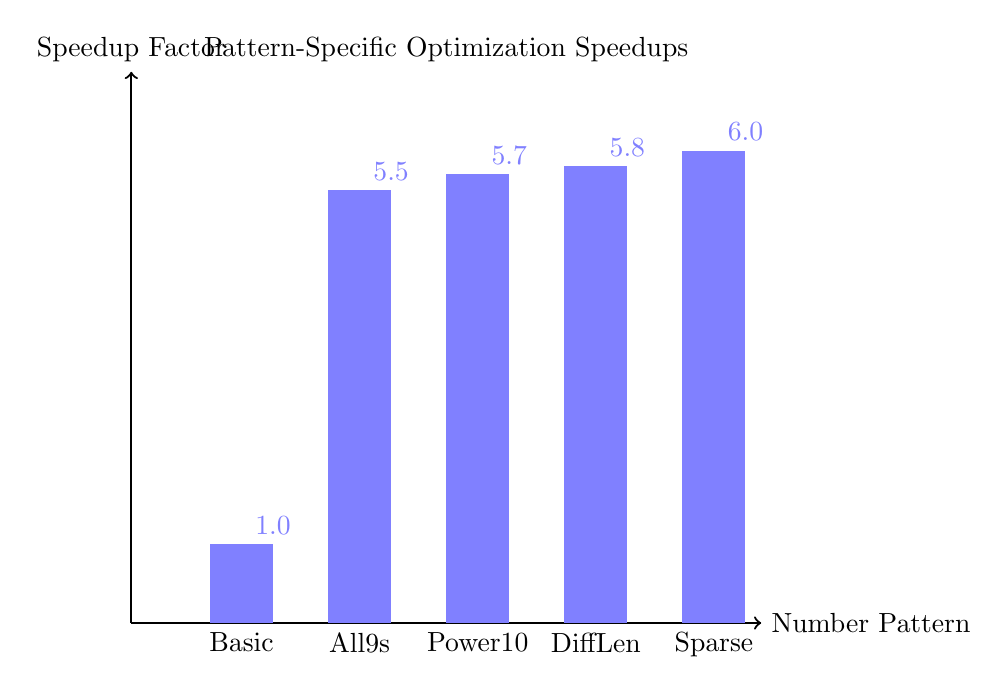
\begin{tikzpicture}
        % Simple bar chart using basic TikZ
        % Set up the axes
        \draw[thick, ->] (0,0) -- (8,0) node[right] {Number Pattern};
        \draw[thick, ->] (0,0) -- (0,7) node[above] {Speedup Factor};
        
        % Draw bars
        \fill[blue!50] (1,0) rectangle (1.8,1) node[above] {1.0};
        \fill[blue!50] (2.5,0) rectangle (3.3,5.5) node[above] {5.5};
        \fill[blue!50] (4,0) rectangle (4.8,5.7) node[above] {5.7};
        \fill[blue!50] (5.5,0) rectangle (6.3,5.8) node[above] {5.8};
        \fill[blue!50] (7,0) rectangle (7.8,6.0) node[above] {6.0};
        
        % X-axis labels
        \node[below] at (1.4,0) {Basic};
        \node[below] at (2.9,0) {All9s};
        \node[below] at (4.4,0) {Power10};
        \node[below] at (5.9,0) {DiffLen};
        \node[below] at (7.4,0) {Sparse};
        
        % Title
        \node[above] at (4,7) {Pattern-Specific Optimization Speedups};
    \end{tikzpicture}
    \caption{Performance improvements with pattern recognition optimizations}
    \label{fig:pattern_speedups}
\end{figure}

For pattern-specific optimizations, our benchmarks have shown impressive speedups ranging from 3.8x to 6.3x across different number patterns, with particularly strong results for:

\begin{itemize}
    \item All-nines patterns (5.5x speedup)
    \item Power-of-ten patterns (5.4-5.9x speedup)
    \item Different-length patterns (5.2-6.2x speedup)
    \item Sparse numbers (3.8-6.3x speedup)
\end{itemize}
>>>>>>> 81a8f8d (Added the argument for resource sensitive interpretability)
